\documentclass{beamer}
%\usepackage[utf8]{inputenc}
\usepackage{textcomp}
%\usepackage{graphicx}
%\usepackage {mathtools}
%\usepackage{utopia} %font utopia imported
\usetheme{CambridgeUS}
%\usecolortheme{default}
\usepackage{minted}
%\usefonttheme{professionalfonts}
%\usepackage{natbib}
%\usepackage{hyperref}
\usepackage{colortbl}
\usepackage{pifont} % Custom bullets
%------------------------------------------------------------
% set colors
\definecolor{greyColor}{RGB}{242,242,245} % grey
\definecolor{greenColor}{RGB}{51,112,98} % green
\definecolor{yellowColor}{RGB}{246,202,84} % yellow
\definecolor{blackColor}{RGB}{84,84,84} % yellow
%------------------------------------------------------------
\setbeamercolor*{palette primary}{bg=yellowColor}
\setbeamercolor*{palette secondary}{bg=greyColor}
\setbeamercolor*{palette tertiary}{bg=greenColor, fg = white}
\setbeamercolor*{titlelike}{fg=greyColor}
\setbeamercolor*{title}{bg=greenColor, fg = white}
\setbeamercolor*{item}{fg=blackColor}
\setbeamercolor*{caption}{fg=greenColor}
\setbeamercolor{frametitle}{fg=black,bg=greyColor}

% customize the caption
\setbeamerfont{caption}{size=\footnotesize}
\setbeamercolor{caption}{fg=blackColor}
\setbeamercolor{caption name}{fg=greenColor}

% https://latex-beamer.com/tutorials/blocks/
\setbeamertemplate{blocks}[rounded][shadow=true]
\setbeamercolor{block title}{bg=greenColor, fg=white}
\setbeamercolor{block body}{bg=greyColor, fg=blackColor}

% see https://pygments.org/styles/
\usemintedstyle{solarized-light}
% [bgcolor=greyColor,linenos, breaklines,frame=leftline, numbersep=1pt,mathescape]
\setminted[shell]{bgcolor=greyColor, breaklines, numbersep=1pt,mathescape, fontsize=\footnotesize}
\setminted[rust]{bgcolor=greyColor,linenos, breaklines,frame=leftline, numbersep=1pt,mathescape, fontsize=\footnotesize}
\setminted[toml]{bgcolor=greyColor,linenos, breaklines,frame=leftline, numbersep=1pt,mathescape, fontsize=\footnotesize}
%------------------------------------------------------------
\title[Rust-Lang]{Rust Programming Language}
\author[Yumcoder]{Yumcoder}

\institute[UoT]{University of Toronto}
\date[{\today} ]
{\today}
%------------------------------------------------------------
%This block of commands puts the table of contents at the 
%beginning of each section and highlights the current section:
%\AtBeginSection[]
%{
	%  \begin{frame}
		%    \frametitle{Contents}
		%    \tableofcontents[currentsection]
		%  \end{frame}
	%}
\AtBeginSection[]{
	\begin{frame}
		\vfill
		\centering
		\begin{beamercolorbox}[sep=8pt,center,shadow=true,rounded=true]{title}
			\usebeamerfont{title}\insertsectionhead\par%
		\end{beamercolorbox}
		\vfill
	\end{frame}
}
%------------------------------------------------------------

\begin{document}
	
	%The next statement creates the title page.
	\frame{\titlepage}
	\begin{frame}
		\frametitle{Contents}
		\mbox{
			\linespread{2.3}
			\tiny
			\begin{columns}
				\column{0.5\textwidth}
				\tableofcontents[sections = 1-10]
				\column{0.5\textwidth}
				\tableofcontents[sections = 11-20]
			\end{columns}
		}
	\end{frame}
	%------------------------------------------------------------
	\section{Introduction}
	\begin{frame}[fragile]
		\frametitle{Installing rustup on Linux or macOS}
		If you’re using Linux or macOS, open a terminal and enter the following command:
		
		\inputminted{shell}{./code/install.shell}
		If the install is successful, the following line will appear:
		\begin{minted}[linenos=false, breaklines,frame=none]{shell}
			Rust is installed now. Great!
		\end{minted}
		To check whether you have Rust installed correctly, open a shell and enter this line:
		\inputminted{shell}{./code/install-check.shell}
	\end{frame}
	
	\begin{frame}[fragile]
		\frametitle{Updating, Uninstalling and Local Documentation}
		Once Rust is installed via rustup, when a new version of Rust is released, updating to the latest version is easy. From your shell, run the following update script:
		
		\inputminted{shell}{./code/install-update.shell}
		
		To uninstall Rust and rustup, run the following uninstall script from your shell:
		\inputminted{shell}{./code/install-uninstall.shell}
		
		The installation of Rust also includes a local copy of the documentation, so you can read it offline. Run \mintinline{shell}{rustup doc}  to open the local documentation in your browser.
	\end{frame}
	
	\begin{frame}[fragile]
		\frametitle{Hello, World!}
		Open a terminal and enter the following commands:
		
		\inputminted[linenos, breaklines,frame=leftline, numbersep=1pt]{shell}{./code/hello-world.shell}
		
		Make a new source file and save it as main.rs:
		\inputminted{rust}{./code/hello-world-main.rs}
		
		Compile and run the file:
		\inputminted{shell}{./code/hello-world-compile.shell}
	\end{frame}
	
	\begin{frame}[fragile]
		\frametitle{Cargo}
		\begin{itemize}
			\item Cargo is \textbf{Rust’s build system and package manager}. 
			\item Most \textbf{Rustaceans} use this tool to manage their Rust projects because Cargo handles a lot of tasks for you, such as building your code, downloading the libraries your code depends on, and building those libraries. 
			\begin{itemize}
				\item[\ding{43}] \textbf{Rustaceans} are people who use Rust, contribute to Rust, or are interested in the development of Rust.
			\end{itemize}
			\item  Cargo comes installed with Rust if you used the official installer.
			\begin{itemize}
				\item[] \inputminted{shell}{./code/cargo.shell}
			\end{itemize}
		\end{itemize}
	\end{frame}
	
	\begin{frame}[fragile]
		\frametitle{Hello, Cargo!}
		Creating a Project with Cargo:
		\inputminted{shell}{./code/hello-cargo.shell}
		
		\begin{figure}
			\centering
			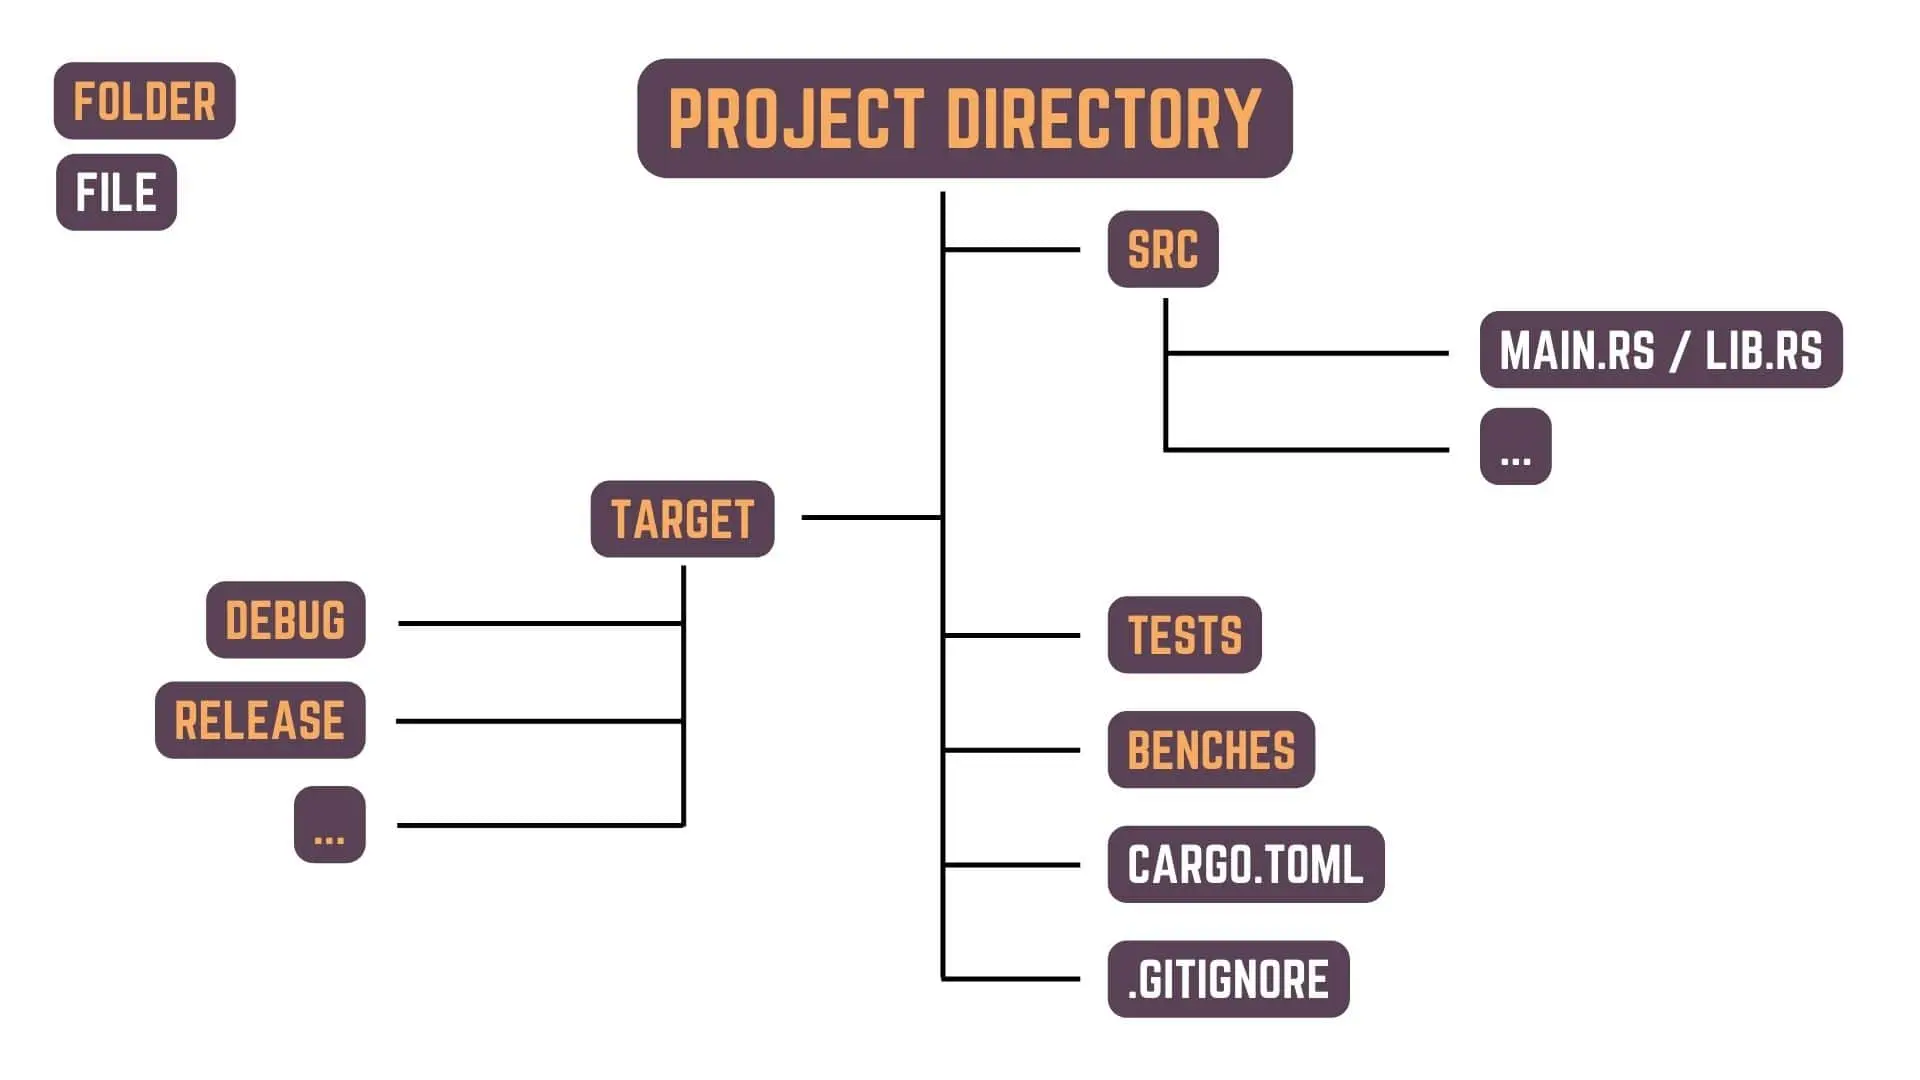
\includegraphics[width=0.65\textwidth]{./img/rust-project-folder-structure.png}
			\caption{Folder structure for projects in rust programming language.}
			\label{fig:folderRustLang}
		\end{figure}
	\end{frame}
	
	\begin{frame}[fragile]
		\frametitle{Cargo.toml}
		This file is in the \textbf{TOML} (Tom’s Obvious, Minimal Language) format, which is \textbf{Cargo’s configuration} format.
		
		\inputminted{toml}{./code/cargo.toml}
	\end{frame}
	
	\begin{frame}[fragile]
		\frametitle{Building and Running a Cargo Project}
		Now open src/main.rs and take a look:
		\inputminted{rust}{./code/hello-world-main.rs}
		
		Build your project by entering the following command:
		
		\inputminted{shell}{./code/hello-world-build.shell}
		
		\begin{itemize}
			\item Use \mintinline{shell}{cargo run} to compile and then run (all in one command).
			\item When your project is finally ready for release, you can use \mintinline{shell}{cargo build --release} to compile it with optimizations (create an executable in target/release instead of target/debug). 
		\end{itemize}
	\end{frame}
	
	\section{Common Programming Concepts}
	
	\begin{frame}{Variables and Mutability}
		\begin{itemize}
			\item by default variables are \textbf{immutable}. 
			\item This is one of many \textbf{\href{https://en.wikipedia.org/wiki/Nudge_theory}{\underline{nudges}} Rust}   gives you to write your code in a way that takes advantage of the \textbf{safety and easy concurrency }that Rust offers. 
			\begin{itemize}
				\item However, you still have the option to make your variables \textbf{mutable}. 
			\end{itemize}
		\end{itemize}
	\end{frame}
	
	\begin{frame}[fragile]
		\frametitle{Immutable variables}
		When a variable is immutable, \textit{once a value is bound to a name, you can’t change that value.}
		
		\inputminted{rust}{./code/immutable-variable.rs}
	\end{frame}
	
	\begin{frame}[fragile]
		\frametitle{Immutable variables (2)}
		You should receive an error message, as shown in this output:
		
		\inputminted{shell}{./code/immutable-variable.shell}
	\end{frame}
	
	\begin{frame}[fragile]
		\frametitle{Mutable variables}
		Although variables are immutable by default, you can make them mutable by adding \mintinline{rust}{mut} in front of the variable name.
		
		\inputminted{rust}{./code/mutable-variable.rs}
	\end{frame}
	
	\begin{frame}[fragile]
		\frametitle{Mutable variables (2)}
		\inputminted{shell}{./code/mutable-variable.shell}
	\end{frame}
	
	\begin{frame}[fragile]
		\frametitle{Constants}
		Rust’s naming convention for constants is to use \textit{all uppercase with underscores between words}.
		\inputminted[linenos=false, frame=none]{rust}{./code/const.rs}
		Like immutable variables, constants are values that are bound to a name and are not allowed to change, but there are a few differences between constants and variables.
		
		\begin{itemize}
			\item you aren’t allowed to use \mintinline{rust}{mut} with constants. Constants aren’t just immutable by default—\textbf{they’re always immutable}. You declare constants using the const keyword instead of the let keyword, and \textbf{the type of the value must be annotated}.
			
			\item 		constants may be set only to a constant expression, \textbf{not the result of a value that could only be computed at runtime}.
		\end{itemize}
	\end{frame}
	
	\begin{frame}[fragile]
		\frametitle{Shadowings}
		Rustaceans say that the first variable is shadowed by the second, which means that the second variable is what the compiler will see when you use the name of the variable.  We can shadow a variable by using the same variable’s name and repeating the use of the \mintinline{rust}{let} keyword as follows
		
		\inputminted{rust}{./code/shadowing.rs}
	\end{frame}
	
	\begin{frame}[fragile]
		\frametitle{Shadowing (2)}
		\inputminted{shell}{./code/shadowing.shell}
	\end{frame}
	
	\begin{frame}[fragile]
		\frametitle{Shadowing vs Mutable variables}
		
		We’re effectively creating a new variable when we use the let keyword again, we can change the type of the value but reuse the same name.
		
		\begin{columns}
			\column{0.5\textwidth}
			\inputminted{rust}{./code/shadowing-vs-mutable-var1.rs}
			The first spaces variable is a string type and the second spaces variable is a number type. 
			\column{0.5\textwidth}
			\inputminted{rust}{./code/shadowing-vs-mutable-var2.rs}
			we’ll get a \textbf{compile-time error}: mismatched types, expected `\&str`, found `usize`.
		\end{columns}
	\end{frame}
	
	\begin{frame}[fragile]
		\frametitle{Data Types - Primitive type}
		\begin{columns}
			\column{0.5\textwidth}
			Data type subsets: 
			\begin{itemize}
				\item Scalar
				\begin{itemize}
					\item Integers
					\item Floating-point numbers
					\item Booleans
					\item Characters
				\end{itemize}
				\item Compound
				\begin{itemize}
					\item Tuples 
					\item Arrays
				\end{itemize}
			\end{itemize}
			\column{0.5\textwidth}
			\inputminted{rust}{./code/data-types.rs}
		\end{columns}
		
		\begin{block}{Statically typed language}
			Keep in mind that Rust is a statically typed language, which means that \textbf{it must know the types of all variables at compile time}. 
		\end{block}
		
		The compiler can usually \textbf{infer} what type we want to use based on the value and how we use it (example: \mintinline{rust}{let x = 2.0; // f64}).
		
	\end{frame}
	
	\begin{frame}[fragile]
		\frametitle{Integer Types}
		\begin{itemize}
			\item An integer is a number without a fractional component.
			\item This type declaration indicates that the value it’s associated with should be an unsigned integer (signed integer types start with \textbf{i}, instead of \textbf{u}) that takes up 32 bits of space.
		\end{itemize}
		
		\begin{table}
			\begin{tabular}{|c|c|c|}
				\hline
				\rowcolor{greyColor}
				Length & Signed & Unsigned \\
				\hline
				8-bit & i8 & u8 \\
				16-bit & i16 & u16 \\
				32-bit & i32 & u32 \\
				64-bit & i64 & u64 \\
				128-bit & i128 & u128 \\
				arch\footnote{the isize and usize types depend on the architecture: 64 bits if you’re on a 64-bit architecture and 32 bits if you’re on a 32-bit architecture.} & isize & usize \\
				\hline
			\end{tabular}
		\end{table}
		
	\end{frame}
	
	\begin{frame}[fragile]
		\frametitle{Integer literals}
		\begin{itemize}
			\item A number literal is a type suffix, such as \mintinline{rust}{57u8}, to designate the type
			\item Number literals can also use \mintinline{rust}{_} as a visual separator to make the number easier to read, such as  \mintinline{rust}{1_000} , which will have the same value as if you had specified \mintinline{rust}{1000}
		\end{itemize}
		\begin{table}
			\begin{tabular}{|c|c|}
				\hline
				\rowcolor{greyColor}
				Number literals	& Example \\
				\hline
				Decimal & \mintinline{rust}{let x = 98_222} \\
				Hex & \mintinline{rust}{let x = 0xff} \\
				Octal & \mintinline{rust}{let x = 0o77} \\
				Binary & \mintinline{rust}{let x = 0b1111_0000} \\
				Byte (u8 only) & \mintinline{rust}{let x = b'A'} \\
				\hline
			\end{tabular}
		\end{table}
	\end{frame}
	
	\begin{frame}[fragile]
		\frametitle{Integer Overflow}
		\begin{itemize}
			\item Let’s say you have a variable of type u8 that can hold values between 0 and 255. 
			\item 		If you try to change the variable to a value outside of that range, such as 256, integer overflow will occur, which can result in one of two behaviors:
			\begin{itemize}
				\item When you’re compiling in \textbf{debug mode}, Rust includes checks for integer overflow that cause your program to panic at runtime if this behavior occurs.
				\item 		When you’re compiling in \textbf{release mode} with the --release flag, Rust does not include checks for integer overflow that cause panics (In the case of a u8, the value 256 becomes 0, the value 257 becomes 1, and so on).
			\end{itemize}
		\end{itemize}
	\end{frame}
	
	\begin{frame}[fragile]
		\frametitle{Floating-Point Types}
		\begin{itemize}
			
			\item Rust’s floating-point types are f32 (32 bits) and f64(64 bits), see (\href{https://en.wikipedia.org/wiki/IEEE_754}{\textsc{IEEE-754 standard}}).
			
			\item The default type is f64 because on modern CPUs it’s roughly the same speed as f32 but is capable of more precision. 
			\item All floating-point types are signed.
		\end{itemize}
		\begin{columns}
			\column{0.5\textwidth}
			\inputminted{rust}{./code/floating-types.rs}
			\column{0.5\textwidth}
			\inputminted{rust}{./code/IEEE-754.rs}
		\end{columns}
	\end{frame}
	
	\begin{frame}[fragile]
		\frametitle{Numeric Operations}
		\inputminted{rust}{./code/numeric-operations.rs}
	\end{frame}
	
	\begin{frame}[fragile]
		\frametitle{Boolean Types}
		Booleans are one byte in size.
		
		\inputminted{rust}{./code/bool-types.rs}
	\end{frame}
	
	
	\begin{frame}[fragile]
		\frametitle{Character Types}
		\begin{itemize}
			\item Note that we specify char literals with \textbf{single quotes}, as opposed to string literals, which use double quotes. 
			\item \textbf{Rust’s char type is four bytes in size} and represents a Unicode Scalar Value, which means it can represent a lot more than just ASCII.
		\end{itemize}
		\begin{figure}
			\centering
			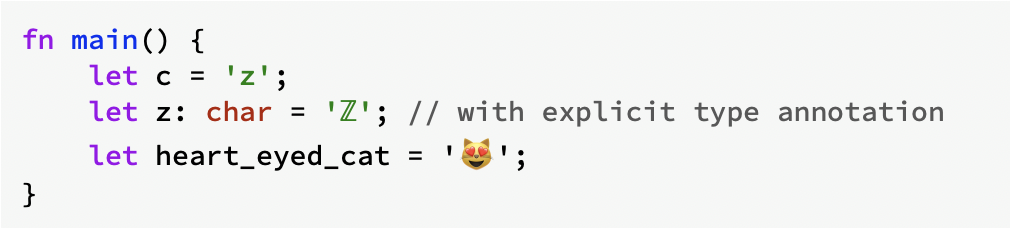
\includegraphics[width=0.65\textwidth]{./img/char.png}
		\end{figure}
	\end{frame}
	
	\begin{frame}[fragile]
		\frametitle{Tuple Types}
		A tuple is a general way of grouping together a number of values with a variety of types into one \textbf{compound type}.
		
		\inputminted{rust}{./code/tuple-types.rs}
	\end{frame}
	
	\begin{frame}[fragile]
		\frametitle{Array Types}
		\begin{itemize}
			\item Another way to have a collection of multiple values is with an array. 
			\item Unlike a tuple, every element of \textbf{an array must have the same type}. 
			\item Unlike arrays in some other languages, \textbf{arrays in Rust have a fixed length}.
			\item \textbf{Rust panics if index out of bounds}.
		\end{itemize}
		\begin{block}{Note}
			Arrays are useful when you want your data allocated on the \textbf{stack} rather than the \textbf{heap} 
		\end{block}
		
		%\inputminted{rust}{./code/tuple-types.rs}
	\end{frame}
	
	\begin{frame}[fragile]
		\frametitle{Array Types (2)}
		
		\inputminted{rust}{./code/array.rs}
	\end{frame}
	
	\begin{frame}[fragile]
		\frametitle{Functions}
		Rust code uses \textbf{snake case} as the conventional style for function and variable names, in which all letters are lowercase and underscores separate words.
		
		\inputminted{rust}{./code/function.rs}
		
		\tiny
		functions \textbf{parameters} are special variables that are part of a function’s signature. When a function has parameters, you can provide it with concrete values for those parameters. Technically, the concrete values are called \textbf{arguments}, but in casual conversation, people tend to use the words parameter and argument interchangeably.
		
	\end{frame}
	
	\begin{frame}[fragile]
		\frametitle{Statements vs Expressions}
		\begin{columns}
			\column{0.4\textwidth}
			\begin{block}{Statements}
				are instructions that perform some action and do not return a value.
			\end{block}
			\column{0.5\textwidth}
			\begin{block}{Expressions}
				evaluate to a resulting value.
			\end{block}
		\end{columns}
		\inputminted{rust}{./code/statements-expressions.rs}
	\end{frame}
	
	
	\begin{frame}[fragile]
		\frametitle{Functions with Return Values}
		\begin{itemize}
			\item Function bodies are made up of a series of statements optionally ending in an expression.
			\item Calling a function is an expression.
			\item Functions can return values to the code that calls them. 
			\item We don’t name return values, but we must declare their type after an arrow (\mintinline{rust}| ->|). 
			\item In Rust, the \textbf{return value of the function} is synonymous with \textbf{the value of the final expression in the block of the body} of a function. 
			\item You can return early from a function by using the return keyword and specifying a value, but most functions return the last expression implicitly.
		\end{itemize}
	\end{frame}
	
	\begin{frame}[fragile]
		\frametitle{Functions with Return Values (2)}
		\inputminted{rust}{./code/function-return.rs}
	\end{frame}
	
	\begin{frame}[fragile]
		\frametitle{Functions with Return Values (3)}
		\inputminted{rust}{./code/function-return2.rs}
		
		The definition of the function \mintinline{rust}|plus_one|  says that it will return an \mintinline{rust}|i32| , but statements don’t evaluate to a value, which is expressed by \mintinline{rust}|()|, the unit type.
	\end{frame}
	
	\begin{frame}[fragile]
		\frametitle{Functions with Return Values (4)}
		\inputminted{shell}{./code/function-return3.shell}
	\end{frame}
	
	\begin{frame}[fragile]
		\frametitle{if Expressions}
		if expressions are sometimes called arms
		\inputminted{rust}{./code/if.rs}
	\end{frame}
	
	\begin{frame}[fragile]
		\frametitle{if Expressions (2)}
		It’s also worth noting that the condition in this code must be a bool. If the condition isn’t a bool, we’ll get an error.
		\begin{columns}
			\column{0.5\textwidth}
			\inputminted{rust}{./code/if-err.rs}
			
			\column{0.5\textwidth}
			\inputminted{rust}{./code/if-err-correct.rs}
		\end{columns}
		\inputminted{shell}{./code/if-err.shell}
	\end{frame}
	
	\begin{frame}[fragile]
		\frametitle{Using if in a let Statement}
		Remember that blocks of code evaluate to the last expression in them, and numbers by themselves are also expressions
		\inputminted{rust}{./code/if-let.rs}
		
		The results of both the if arm and the else arm should be in the same type. So, \mintinline{rust}|let number = if condition { 5 } else { "six" };| get panic error.
	\end{frame}
	
	
	\begin{frame}[fragile]
		\frametitle{Repetition with Loops}
		The loop keyword tells Rust to execute a block of code over and over again forever or until you explicitly tell it to stop.
		\inputminted{rust}{./code/loop.rs}
	\end{frame}
	
	\begin{frame}[fragile]
		\frametitle{Returning Values from Loops}
		\inputminted{rust}{./code/loop-return.rs}
	\end{frame}
	
	\begin{frame}[fragile]
		\frametitle{Loop Labels to Disambiguate Between Multiple Loops}
		Loop labels must begin with a single quote
		\scriptsize
		\inputminted{rust}{./code/loop-label.rs}
	\end{frame}
	
	\begin{frame}[fragile]
		\frametitle{Conditional Loops with while}
		\inputminted{rust}{./code/while.rs}
	\end{frame}
	
	\begin{frame}[fragile]
		\frametitle{Repetition with for}
		\inputminted{rust}{./code/for.rs}
	\end{frame}
	
	\begin{frame}[fragile]
		\frametitle{for with range}
		\inputminted{rust}{./code/for-range.rs}
	\end{frame}
	
	\section{Understanding Ownership}
	
	\begin{frame}[fragile]
		\frametitle{What Is Ownership?}
		\begin{itemize}
			\item \textbf{Ownership} is a set of rules that governs how a Rust program manages memory.
			\item 		Some languages have \textbf{garbage collection} that \textbf{regularly looks} (performance?) for no-longer used memory as the program runs;
			\item 		 In other languages, the \textbf{programmer} must \textbf{explicitly allocate and free} the memory.
			\item 		 Rust uses a third approach: memory is managed through a system of ownership with \textbf{a set of rules} that the\textbf{ compiler checks}. If any of the rules are violated, the program won’t compile.
		\end{itemize}
		\begin{block}{Note}
			None of the features of ownership will slow down your program while it’s running.
		\end{block}
		\tiny Because ownership is a new concept for many programmers, it does take some time to get used to.
	\end{frame}
	
	
	\begin{frame}[fragile]
		\frametitle{The Stack and the Heap}
		\begin{itemize}
			\item In a systems programming language like Rust, whether a value is on the stack or the heap affects how the language behaves and why you have to make certain decisions. Parts of ownership will be described in relation to the stack and the heap later in the following, so here is a brief explanation.
			\item 	Both the \textbf{stack and the heap} are \textbf{parts of memory} available to your code to use at runtime, but they are structured in different ways. 
			\item The \textbf{stack} stores values in the order it gets them and removes the values in the opposite order. This is \textbf{referred to as last in, first out}. Adding data is called pushing onto the stack, and removing data is called popping off the stack. \textbf{All data stored on the stack must have a known, fixed size}. Data with an unknown size at compile time or a size that might change must be stored on the heap instead.
		\end{itemize}
	\end{frame}
	
	\begin{frame}[fragile]
		\frametitle{The Stack and the Heap (2)}
		\begin{itemize}
			\item 	The heap is less organized: when you put data on the heap, you request a certain amount of space. The \textbf{memory allocator} finds an empty spot in the heap that is big enough, marks it as being in use, and returns a pointer, which is the address of that location. This process is called allocating on the heap and is sometimes abbreviated as just allocating (pushing values onto the stack is not considered allocating). \textbf{Because the pointer to the heap is a known, fixed size, you can store the pointer on the stack, but when you want the actual data, you must follow the pointer}.
			\item 	\textbf{Pushing to the stack is faster than allocating on the heap} because the allocator never has to search for a place to store new data; that location is always at the top of the stack. Comparatively, allocating space on the heap requires more work, because the allocator must first find a big enough space to hold the data and then perform bookkeeping to prepare for the next allocation.
			
		\end{itemize}
	\end{frame}
	
	
	
	\begin{frame}[fragile]
		\frametitle{The Stack and the Heap (3)}
		\begin{itemize}
			\item 	When your code calls a function, the values passed into the function (including, potentially, pointers to data on the heap) and the function’s local variables get pushed onto the stack. When the function is over, those values get popped off the stack.
			\item 	Keeping track of what parts of code are using what data on the heap, minimizing the amount of duplicate data on the heap, and cleaning up unused data on the heap so you don’t run out of space are all problems that ownership addresses. Once you understand ownership, you won’t need to think about the stack and the heap very often, but knowing that the main purpose of ownership is to manage heap data can help explain why it works the way it does.
		\end{itemize}
	\end{frame}
	
	\begin{frame}[fragile]
		\frametitle{Ownership Rules}
		\begin{itemize}
			\item Each value in Rust has an owner.
			\item There can only be one owner at a time.
			\item When the owner goes out of scope, the value will be dropped.
		\end{itemize}
		
	\end{frame}
	
	\begin{frame}[fragile]
		\frametitle{Variable Scope}
		\inputminted{rust}{./code/scope.rs}
	\end{frame}
	
	\begin{frame}[fragile]
		\frametitle{The String Type}
		\begin{itemize}
			\item To illustrate the rules of ownership, we need a data type that is more complex than those we covered in the “Data Types” section
			\item The types covered previously are all a\textbf{ known size}, can be \textbf{stored on the stack and popped off the stack when their scope is over}, and can be quickly and trivially copied to make a new, independent instance if another part of code needs to use the same value in a different scope. 
			\item We want to look at \textbf{data that is stored on the heap} and explore how Rust knows when to clean up that data, and the \textbf{String} type is a great example
		\end{itemize}
	\end{frame}
	
	
	\begin{frame}[fragile]
		\frametitle{The String Type (2)}
		\begin{itemize}
			\item String literals(\mintinline{rust}|&str|) are hard-coded into our program (\textbf{fast and efficient}). String literals are convenient, but they aren’t suitable for every situation in which we may want to use text.
			\begin{itemize}
				\item 	One reason is that they’re \textbf{immutable}. 
				\item 	Another is that not every string value can be known when we write our code (for example, user input) 
			\end{itemize}
			\item 	For these situations, Rust has a second string type, \mintinline{rust}|String|.
			\begin{itemize}
				\item This type manages data allocated on the \textbf{heap} and as such is able to store an amount of text that is unknown to us at compile time.
				\item  You can create a \mintinline{rust}|String| from a string literal using the from function, like so: \mintinline{rust}|let s = String::from("hello");|.
			\end{itemize}
		\end{itemize}
	\end{frame}
	
	\begin{frame}[fragile]
		\frametitle{The String Type (3)}}
	\scriptsize
	\inputminted{rust}{./code/string.rs}
\end{frame}

\begin{frame}[fragile]
	\frametitle{Move}
	\inputminted{rust}{./code/move.rs}
	
	Bind the value 5 to x; then make a copy of the value in x and bind it to y.”  Because \textbf{integers are simple values with a known, fixed size}, and these two 5 values are pushed onto the \textbf{stack}
	
	\begin{block}{Primitive type on stack}
		\textbf{Primitive type}'s size known and fixed  so pushed onto the \textbf{stack}
	\end{block}
	
\end{frame}

\begin{frame}[fragile]
	\frametitle{Move (2)}
	
	\begin{columns}
		\column{0.6\textwidth}
		\inputminted{rust}{./code/move-string.rs}
		\column{0.4\textwidth}
		\begin{figure}
			\centering
			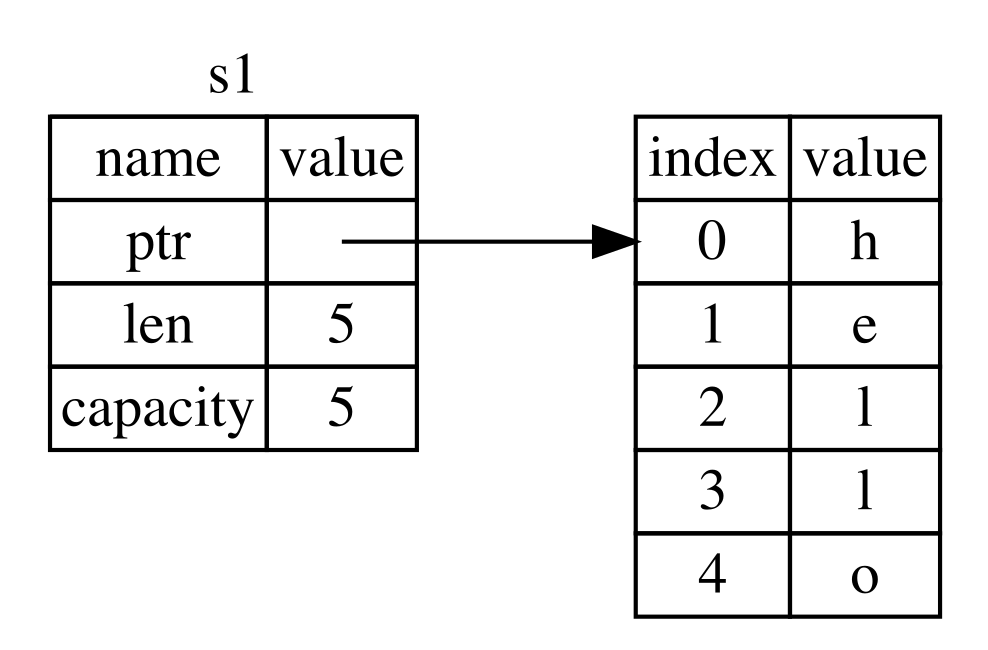
\includegraphics[width=0.65\textwidth]{./img/trpl04-01.png}
			\caption{a String in memory}
			\label{fig:figureS1}
		\end{figure}
	\end{columns}
	
	The second line would make a copy of the value in s1 and bind it to s2. But this isn’t quite what happens.
	
	\textbf{A String is made up of three parts, shown on the left: a pointer to the memory that holds the contents of the string, a length, and a capacity. This group of data is stored on the stack. On the right is the memory on the heap that holds the contents.}
\end{frame}


\begin{frame}[fragile]
	\frametitle{Move (3)}
	When we assign s1 to s2, the String data is copied, meaning we copy the pointer, the length, and the capacity that are on the stack. We do not copy the data on the heap that the pointer refers to. In other words, the data representation in memory looks like the following ( sounds like making a \textbf{shallow copy}):
		\begin{figure}
		\centering
		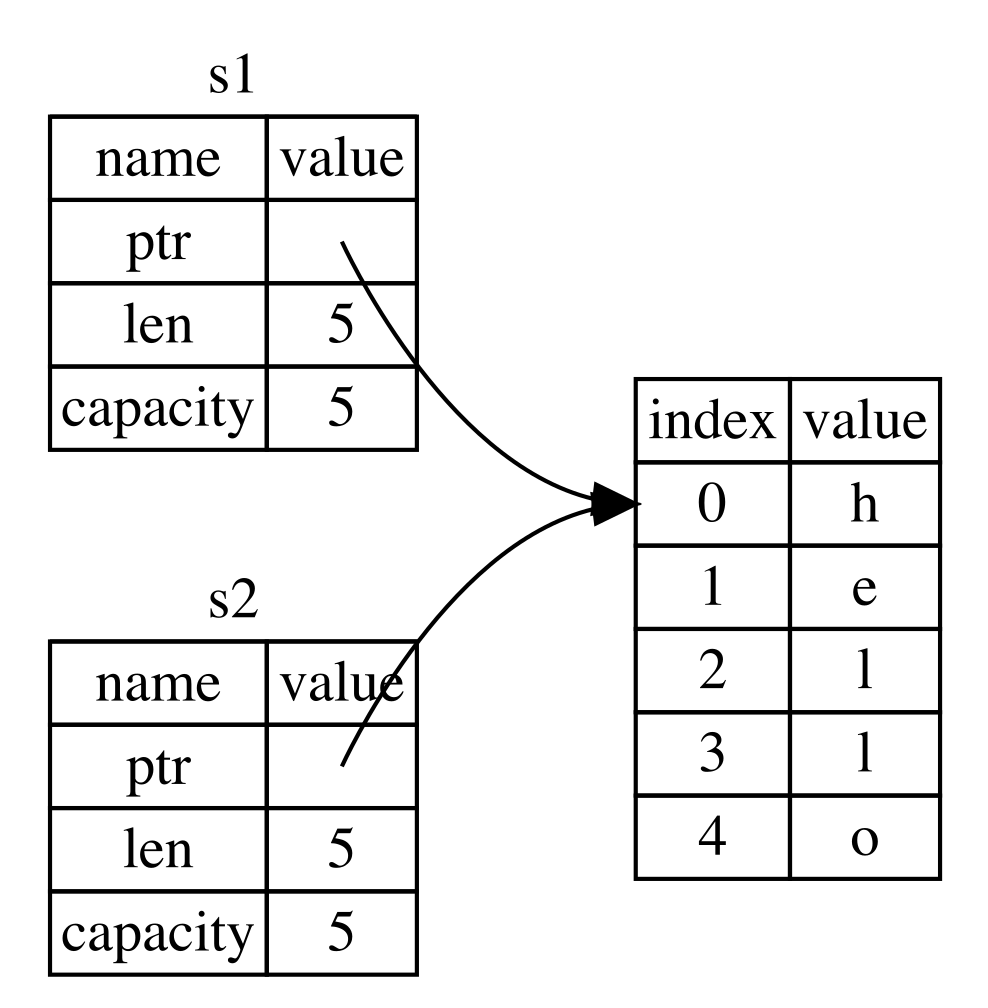
\includegraphics[width=0.3\textwidth]{./img/trpl04-02.png}
		\caption{Representation in memory of the variable s2 that has a copy of the pointer, length, and capacity of s1}
		\label{fig:figureS2}
	\end{figure}
\end{frame}



\begin{frame}[fragile]
	\frametitle{Another possibility for what s2 = s1 might do if Rust copied the heap data as well}
	The representation does not look like the following Figure, which is what memory would look like if Rust instead copied the heap data as well. If Rust did this, the operation s2 = s1 could be very expensive in terms of runtime performance if the data on the heap were large (\textbf{deep copy}).
	\begin{figure}
		\centering
		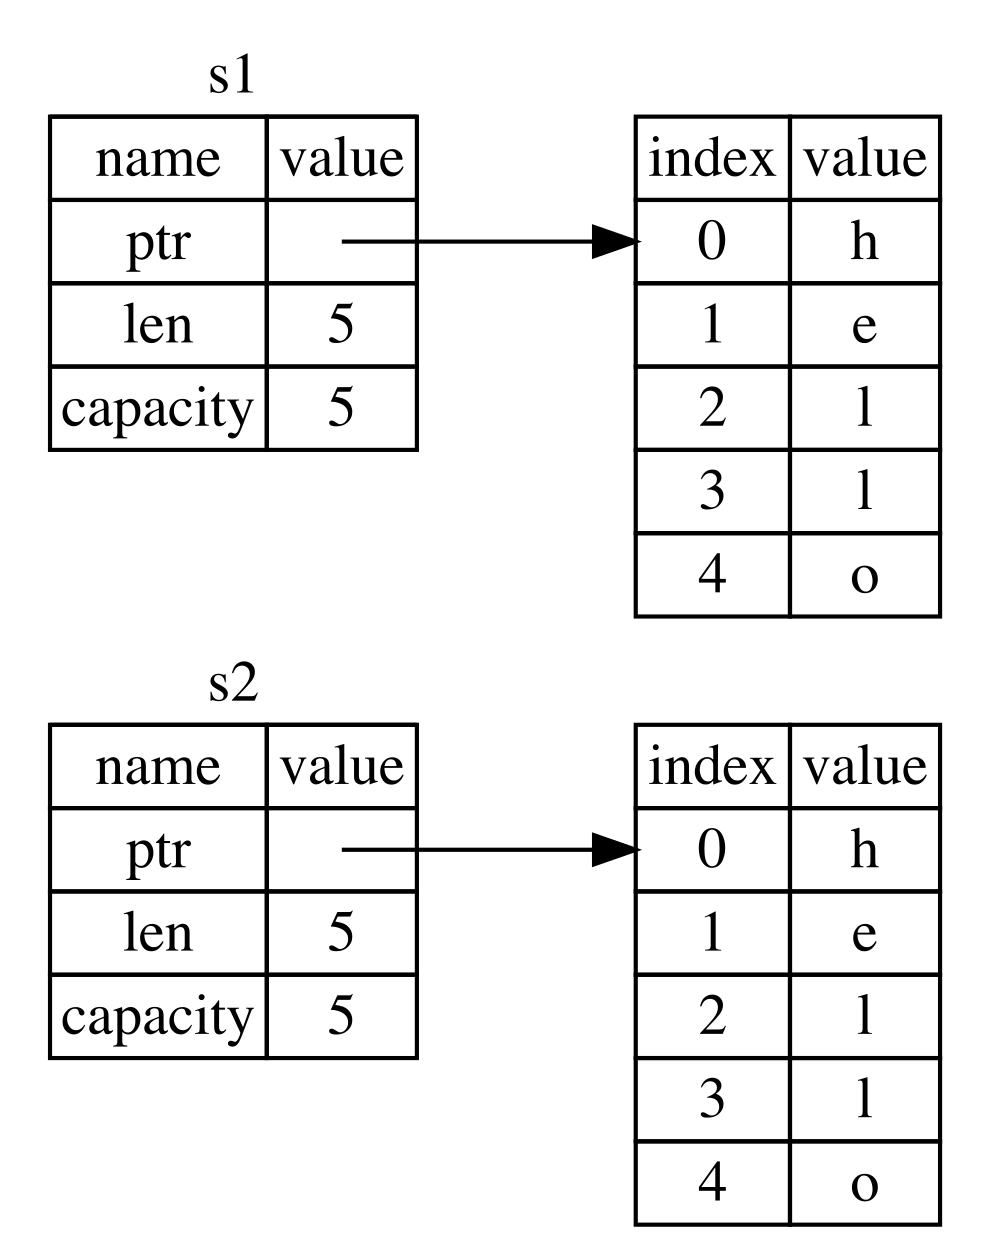
\includegraphics[width=0.3\textwidth]{./img/trpl04-03.png}
		\label{fig:figureSAnotherPossibility}
	\end{figure}
\end{frame}

\begin{frame}[fragile]
	\frametitle{s1 was moved into s2}
\begin{itemize}
	\item When a variable goes out of scope, \textbf{Rust automatically calls the drop function and cleans up the heap memor}y for that variable. 
	\item When s2 and s1 go out of scope, they will both try to free the same memory. This is known as a \textbf{double free error} and is one of the memory safety bugs.
	\item \textbf{Freeing memory twice} can lead to memory corruption, which can potentially lead to security vulnerabilities.
	\item To ensure memory safety, after the line let s2 = s1;, Rust considers s1 as no longer valid. Therefore, Rust doesn’t need to free anything when s1 goes out of scope.
\end{itemize}

\end{frame}

\begin{frame}[fragile]
	\frametitle{s1 was moved into s2 (2)}
			\inputminted{rust}{./code/move-string.rs}
\end{frame}
\begin{frame}[fragile]
	\frametitle{s1 was moved into s2 (3)}
		\inputminted{shell}{./code/move-string.shell}
\end{frame}

\begin{frame}[fragile]
	\frametitle{s1 was moved into s2 (4)}
	If you’ve heard the terms shallow copy and deep copy while working with other languages, the concept of copying the pointer, length, and capacity without copying the data probably sounds like making a shallow copy. But \textbf{because Rust also invalidates the first variable, instead of being called a shallow copy, it’s known as a move}. In this example, we would say that s1 was moved into s2. 
	\begin{figure}
		\centering
		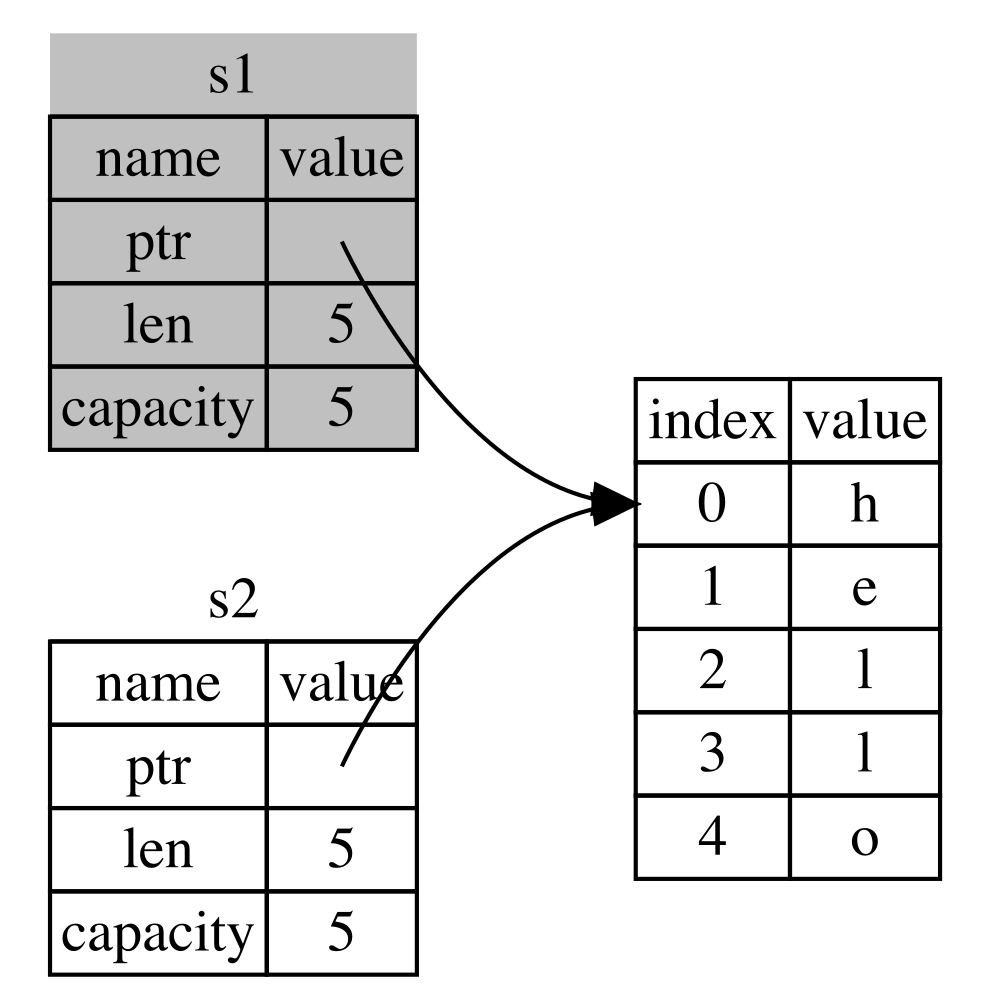
\includegraphics[width=0.3\textwidth]{./img/trpl04-04.png}
		\label{fig:figureMove}
	\end{figure}
\end{frame}

\begin{frame}[fragile]
	\frametitle{Move notes}
			
	\begin{block}{Memory safety bugs}
		That solves our problem! With only s2 valid, when it goes out of scope it alone will free the memory, and we’re done.
	\end{block}
	
			
	\begin{block}{Design choice}
		Rust will never automatically create “deep” copies of your data. Therefore, any automatic copying can be assumed to be inexpensive in terms of runtime performance.
	\end{block}
	
\end{frame}



\begin{frame}[fragile]
	\frametitle{Deeply copy with clone}
	If we do want to deeply copy the heap data of the String, not just the stack data, we can use a common method called clone.
	
		\begin{columns}
		\column{0.6\textwidth}
			\inputminted{rust}{./code/move-clone.rs}
		\column{0.4\textwidth}
			\begin{figure}
				\centering
				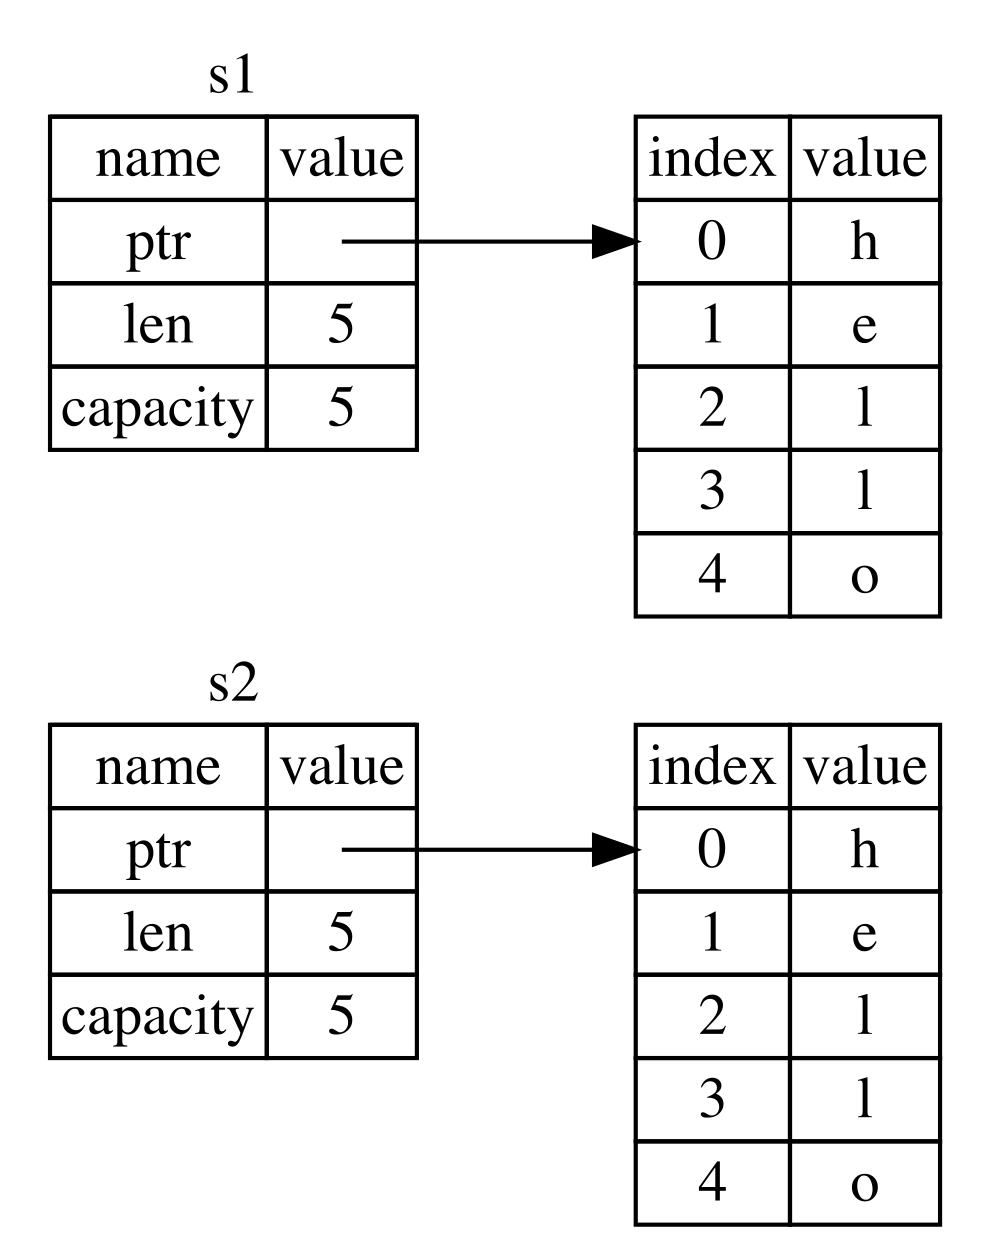
\includegraphics[width=0.8\textwidth]{./img/trpl04-03.png}
				\label{fig:figureSAnotherPossibility2}
			\end{figure}
	\end{columns}
\end{frame}



\begin{frame}[fragile]
	\frametitle{Stack-Only Data: Copy and Clone}
	We don’t have a call to clone, but x is still valid and wasn’t moved into y.
	\inputminted{rust}{./code/move2.rs}

The reason is that types such as integers that have \textbf{a known size at compile time} are stored entirely on the \textbf{stack}, so \textbf{copies of the actual values are quick to make}. That means there’s no reason we would want to prevent x from being valid after we create the variable y. In other words, there’s no difference between deep and shallow copying here, so calling clone wouldn’t do anything different from the usual shallow copying, and we can leave it out.
\end{frame}

\begin{frame}[fragile]
	\frametitle{Ownership and Functions}
	\inputminted[fontsize=\scriptsize]{rust}{./code/ownership-functions.rs}
\end{frame}

\begin{frame}[fragile]
	\frametitle{Return Values and Scope}
	\inputminted[fontsize=\scriptsize]{rust}{./code/ownership-return.rs}
\end{frame}

\begin{frame}[fragile]
	\frametitle{Returning ownership}
	\inputminted{rust}{./code/ownership-return2.rs}
	Rust has a feature for using a value without transferring ownership, called \textbf{\textit{references}}.
\end{frame}

\begin{frame}[fragile]
	\frametitle{References}
	A reference is\textbf{ like a pointer} in that it’s \textbf{an address we can follow to access the data} stored at that address; \textbf{that data is owned by some other variable}. Unlike a pointer,\textbf{ a reference is guaranteed to point to a valid value of a particular type for the life of that reference}.
	\begin{columns}
	\column{0.7\textwidth}
	\inputminted[fontsize=\scriptsize]{rust}{./code/references.rs}
	\column{0.3\textwidth}
		\small
	Note that we pass \&s1 into calculate\_length and, in its definition, we take \&String rather than String. These ampersands represent references, and they allow you to refer to some value without taking ownership of it
\end{columns}

\end{frame}

\begin{frame}[fragile]
	\frametitle{References (2)}
	\inputminted[fontsize=\scriptsize]{rust}{./code/references.rs}
		\begin{figure}
		\centering
		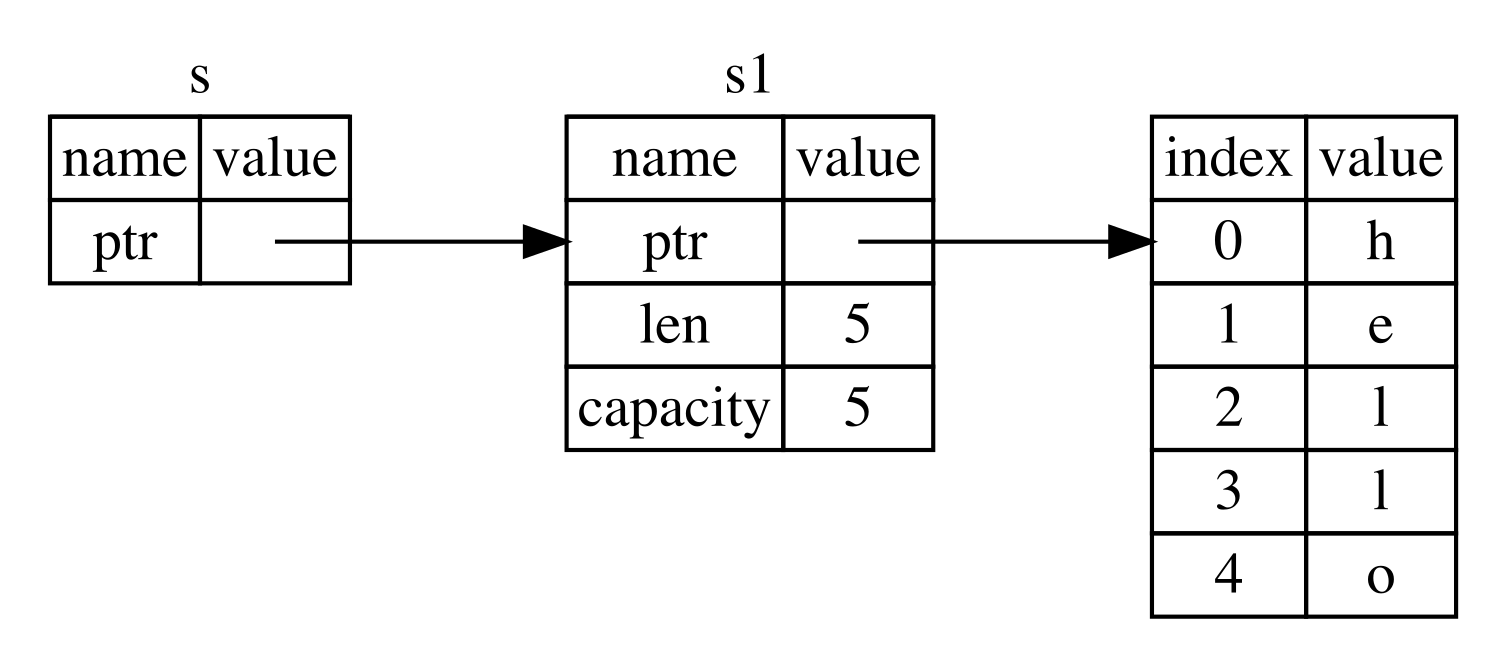
\includegraphics[width=0.6\textwidth]{./img/trpl04-05.png}
		\label{fig:figureRef}
	\end{figure}
\end{frame}

\begin{frame}[fragile]
	\frametitle{Borrowing}
	\textbf{borrowing}: \textit{the action of creating a reference}.
	As in real life, if a person owns something, you can borrow it from them. When you’re done, you have to give it back. You don’t own it. So, what happens if we try to modify something we’re borrowing?
		\inputminted{rust}{./code/borrowing.rs}
		
		\small
	Just as variables are immutable by default, so are references. We’re not allowed to modify something we have a reference to.
\end{frame}

\begin{frame}[fragile]
	\frametitle{Borrowing (2)}
	\inputminted{shell}{./code/borrowing.shell}
\end{frame}


\begin{frame}[fragile]
	\frametitle{Borrowing, Mutable References}
	We can fix the code to allow us to modify a borrowed value with just a few small tweaks that use, instead, a mutable reference (\mintinline{rust}|&mut|).
	\inputminted{rust}{./code/borrowing-mut-ref.rs}
\end{frame}


\begin{frame}[fragile]
	\frametitle{Mutable references restriction}
	\textbf{If you have a mutable reference to a value, you can have no other references to that value}. 
	\inputminted{rust}{./code/borrowing-mut-ref-err1.rs}
\end{frame}

\begin{frame}[fragile]
	\frametitle{Mutable references restriction (2)}
	\inputminted[fontsize=\scriptsize]{shell}{./code/borrowing-mut-ref-err1.shell}
	
	\scriptsize
	This error says that this code is invalid because we cannot borrow s as mutable more than once at a time. The first mutable borrow is in r1 and must last until it’s used in the println!, but between the creation of that mutable reference and its usage, we tried to create another mutable reference in r2 that borrows the same data as r1.
	
\end{frame}

\begin{frame}[fragile]
	\frametitle{Why mutable references restriction exist in Rust?}
	It’s something that new Rustaceans struggle with because most languages let you mutate whenever you’d like. The benefit of having this restriction is that \textbf{Rust can prevent data races at compile time}. 
	
	A data race is similar to a race condition and happens when these three behaviors occur:
	
	\begin{itemize}
		\item Two or more pointers access the same data at the same time.
		\item 	At least one of the pointers is being used to write to the data.
		\item 	There’s no mechanism being used to synchronize access to the data.
	\end{itemize}
Data races cause undefined behavior and can be difficult to diagnose and fix when you’re trying to track them down at runtime.
	
\end{frame}


\begin{frame}[fragile]
	\frametitle{Mutable references restriction example}
As always, we can use curly brackets to create a new scope, allowing for multiple mutable references, just not simultaneous ones:
	\inputminted{rust}{./code/borrowing-simultaneous.rs}
\end{frame}

\begin{frame}[fragile]
	\frametitle{Mutable references restriction example (combining mutable and immutable references)}
	\inputminted{rust}{./code/borrowing-combining.rs}
\end{frame}

\begin{frame}[fragile]
	\frametitle{Mutable references restriction example (combining mutable and immutable references)}
	\inputminted{shell}{./code/borrowing-combining.shell}
\end{frame}

\begin{frame}[fragile]
	\frametitle{Mutable references restriction example (combining mutable and immutable references, note to  reference’s scope)}
	\inputminted{rust}{./code/borrowing-combining-note.rs}
\end{frame}

\begin{frame}[fragile]
	\frametitle{Dangling References}
	In languages with pointers, it’s easy to erroneously create a dangling pointer—\textbf{a pointer that references a location in memory that may have been given to someone else}—by freeing some memory while preserving a pointer to that memory. In Rust, by contrast, \textbf{the compiler guarantees that references will never be dangling references}: if you have a reference to some data, the compiler will ensure that the data will not go out of scope before the reference to the data does.
	\inputminted[fontsize=\scriptsize]{rust}{./code/dangling.rs}
\end{frame}

\begin{frame}[fragile]
	\frametitle{Dangling References (2)}
	
	\inputminted{shell}{./code/dangling.shell}
\end{frame}

\begin{frame}[fragile]
	\frametitle{Dangling References (3), solution}
	The solution here is to return the String directly:
	
	\inputminted{rust}{./code/dangling-sol.rs}
	
	This works without any problems. \textbf{Ownership is moved out, and nothing is deallocated.}
\end{frame}


\begin{frame}[fragile]
	\frametitle{The Slice Type}
	\textbf{Slices} let you \textbf{reference a contiguous sequence of elements in a collection} rather than the whole collection. A slice is \textbf{a kind of reference, so it does not have ownership}.
\end{frame}

\begin{frame}[fragile]
	\frametitle{Learn application of Slice Type by example}
	Here’s a small programming problem: write a function that takes a string of words separated by spaces and returns the first word it finds in that string.
	\scriptsize
	\inputminted[fontsize=\scriptsize]{rust}{./code/slice.rs}
\end{frame}

\begin{frame}[fragile]
	\frametitle{Learn application of Slice Type by example}
\begin{itemize}
	\item This program compiles without any errors and would also do so if we used word after calling s.clear(). Because word isn’t connected to the state of s at all, word still contains the value 5. We could use that value 5 with the variable s to try to extract the first word out, but this would be a bug because the contents of s have changed since we saved 5 in word.
	\item Luckily, Rust has a solution to this problem: string slices.
\end{itemize}
\end{frame}

\begin{frame}[fragile]
	\frametitle{String Slices}
	
		\begin{columns}
		\column{0.6\textwidth}
		\inputminted{rust}{./code/string-slice.rs}
		\column{0.4\textwidth}
		\begin{figure}
			\centering
			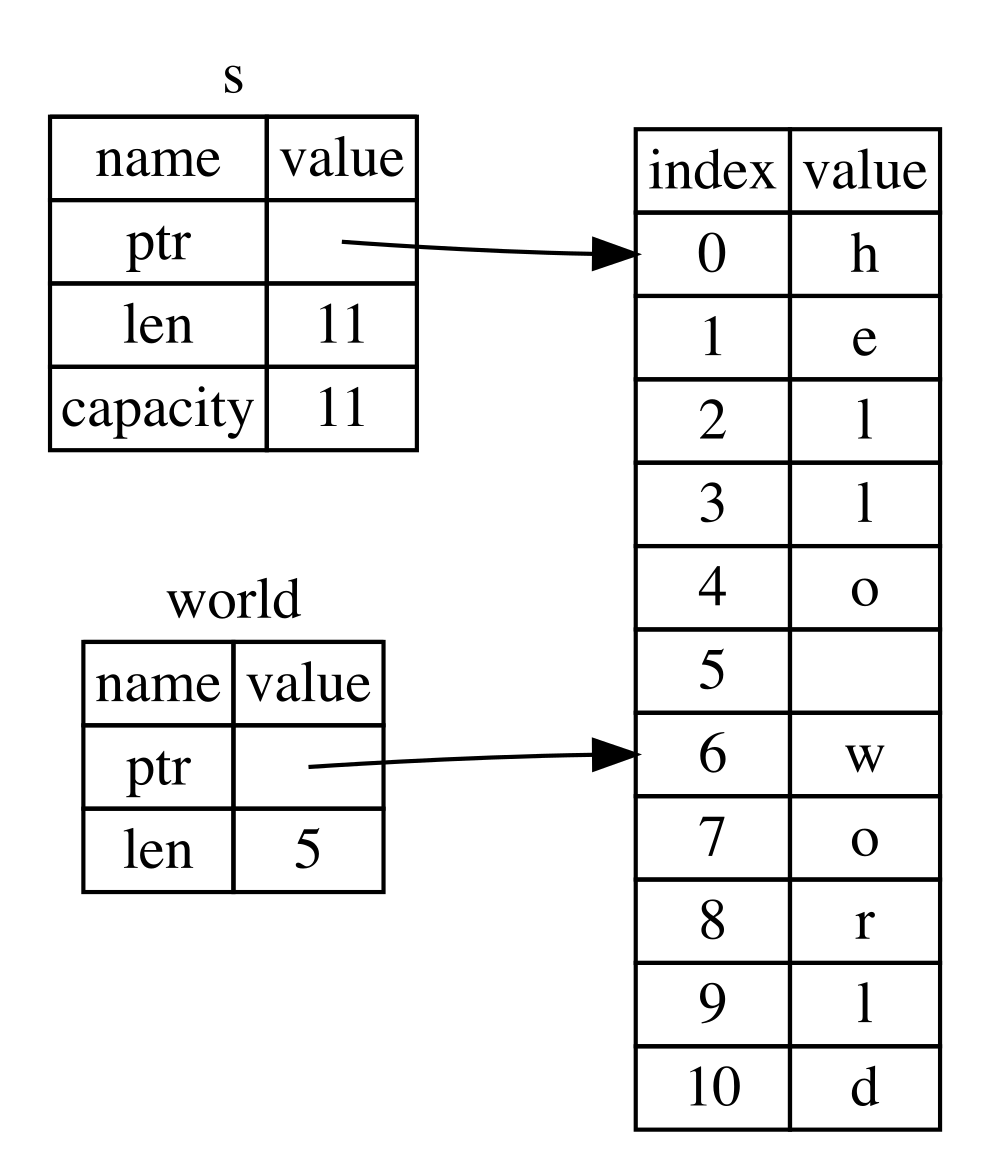
\includegraphics[width=0.8\textwidth]{./img/trpl04-06.png}
		\end{figure}
		
	\end{columns}

\end{frame}

\begin{frame}[fragile]
	\frametitle{Rewrite first\_word to return a slice}
		\inputminted{rust}{./code/slice2.rs}
\end{frame}

\begin{frame}[fragile]
	\frametitle{ Rewrite first\_word to return a slice (2)}
	\inputminted{shell}{./code/slice2.shell}
\end{frame}

\begin{frame}[fragile]
	\frametitle{Rewrite first\_word to return a slice (3)}
	Recall from the borrowing rules that if we have an immutable reference to something, we cannot also take a mutable reference. Because clear needs to truncate the String, it needs to get a mutable reference. The println! after the call to clear uses the reference in word, so the immutable reference must still be active at that point. Rust disallows the mutable reference in clear and the immutable reference in word from existing at the same time, and compilation fails. Not only has Rust made our API easier to use, but it has also eliminated an entire class of errors at compile time!
\end{frame}

\begin{frame}[fragile]
	\frametitle{Improve first\_word function}
	\mintinline{rust}|fn first_word(s: &String) -> &str {/*...*/}| 
	
	A more experienced Rustacean would write the signature as in below instead because it allows us to use the same function on both \mintinline{rust}|&String|  values and  \mintinline{rust}|&str|  values.

	\mintinline{rust}|fn first_word(s: &str) -> &str {/*...*/}| 
\end{frame}


\section{Using Structs to Structure Related Data}

\begin{frame}[fragile]
	\frametitle{Defining and Instantiating Structs}
	\begin{itemize}
		\item A\textbf{ struct, or structure,} is a custom data type that lets you package together and name multiple related values that make up a meaningful group. If you’re familiar with an object-oriented language, a struct is like an\textit{ object’s data attributes}.
		\item 	\textbf{Structs are similar to tuples}, in that both hold multiple related values. Like tuples, the pieces of a struct can be different types. Unlike with tuples, in a struct you’ll name each piece of data so it’s clear what the values mean. Adding these names means that structs are more flexible than tuples: you don’t have to rely on the order of the data to specify or access the values of an instance.
	\end{itemize}
\end{frame}

\begin{frame}[fragile]
	\frametitle{Defining and Instantiating Structs (2)}
\inputminted{rust}{./code/struct.rs}
\end{frame}

\begin{frame}[fragile]
	\frametitle{Using the Field Init Shorthand}
	\inputminted{rust}{./code/field-shorthand.rs}
\end{frame}

\begin{frame}[fragile]
	\frametitle{Creating Instances From Other Instances With Struct Update Syntax}
	\inputminted{rust}{./code/struct-build.rs}
\end{frame}

\begin{frame}[fragile]
	\frametitle{Creating Instances From Other Instances With Struct Update Syntax (2)}
	The ..user1 \textbf{must come last to specify that any remaining fields should get their values from the corresponding fields} in user1.
	
	\begin{block}{Note that the struct update syntax uses = like an assignment}
		This is because it moves the data. In this example, we can no longer use user1 after creating user2 because the String in the username field of user1 was moved into user2. If we had given user2 new String values for both email and username, and thus only used the active and sign\_in\_count values from user1, then user1 would still be valid after creating user2. The types of active and sign\_in\_count are types that implement the Copy trait.
	\end{block}
	
\end{frame}


\begin{frame}[fragile]
	\frametitle{Creating Instances From Other Instances With Struct Update Syntax (3)}
		\inputminted{rust}{./code/struct-err.rs}
\end{frame}


\begin{frame}[fragile]
	\frametitle{Creating Instances From Other Instances With Struct Update Syntax (4)}
	\inputminted{shell}{./code/struct-err2.shell}
\end{frame}

\begin{frame}[fragile]
	\frametitle{Ownership of Struct Data}
	\begin{itemize}
		\item In the User struct definition,\textbf{ we used the owned String type rather than the \mintinline{rust}|&str| string slice type.} This is a deliberate choice because we want each instance of this struct to own all of its data and for that data to be valid for as long as the entire struct is valid.
		\item 	\textbf{It’s also possible for structs to store references to data owned by something else, but to do so requires the use of lifetimes}, a Rust feature that we’ll discuss later. Lifetimes ensure that the data referenced by a struct is valid for as long as the struct is.
	\end{itemize}
\end{frame}


\begin{frame}[fragile]
	\frametitle{Using Tuple Structs without Named Fields to Create Different Types}
	Rust also supports structs that look similar to tuples, called tuple structs. Tuple structs have the added meaning the struct name provides but don’t have names associated with their fields; rather, they just have the types of the fields. Tuple structs are useful when you want to give the whole tuple a name and make the tuple a different type from other tuples, and when naming each field as in a regular struct would be verbose or redundant.
	\inputminted{rust}{./code/tuple-struct.rs}
\end{frame}


\begin{frame}[fragile]
	\frametitle{Unit-Like Structs Without Any Fields}
	You can also define structs that don’t have any fields! These are called \textbf{unit-like structs} because they behave similarly to ().
	\inputminted{rust}{./code/unit-like-struct.rs}
	
	\begin{block}{Unit type}
		The tuple without any values has a special name, unit. This value and its corresponding type are both written () and represent an empty value or an empty return type. Expressions implicitly return the unit value if they don’t return any other value.
	\end{block}
\end{frame}

\begin{frame}[fragile]
	\frametitle{Unit-Like Structs Without Any Fields (2)}
	Unit-like structs can be useful when you need to implement a trait on some type but don’t have any data that you want to store in the type itself. 
	Example, see: The global memory allocator, \href{https://doc.rust-lang.org/src/alloc/alloc.rs.html#59}{\colorbox{lightgray}{Global}}, is a unit struct.
\end{frame}

\begin{frame}[fragile]
	\frametitle{Method Syntax}
	\textbf{Methods} are similar to \textbf{functions}: we declare them with the \mintinline{rust}|fn| keyword and a name, they can have parameters and a return value, and they contain some code that’s run when the method is called from somewhere else. Unlike functions, methods are defined within the context of a struct (or an enum or a trait object, which we cover later), and their \textbf{first parameter is always self}, which represents the instance of the struct the method is being called on.
\end{frame}

\begin{frame}[fragile]
	\frametitle{Method Syntax(2)}
	\inputminted{rust}{./code/method.rs}
\end{frame}

\begin{frame}[fragile]
	\frametitle{Associated Functions}
	\begin{itemize}
		\item \textbf{All functions defined within an \mintinline{rust}|impl|  block} are called associated functions because they’re associated with the type named after the  \mintinline{rust}|impl| . We can define associated functions that don’t have self as their first parameter (and\underline{ thus are not methods}) because they don’t need an instance of the type to work with. We’ve already used one function like this: the String::from function that’s defined on the String type.
		\item 	Associated functions that aren’t methods are often used for constructors that will return \textbf{a new instance of the struct}(factory method). These are often called \textbf{new}, but new isn’t a special name and isn’t built into the language.
	\end{itemize}
\end{frame}

\begin{frame}[fragile]
	\frametitle{Associated Functions}
	\inputminted{rust}{./code/factory-method.rs}
\end{frame}

Multiple impl Blocks

\begin{frame}[fragile]
	\frametitle{Multiple \mintinline{rust}|impl| Blocks}
	\inputminted{rust}{./code/multi-impl.rs}
\end{frame}

\section{Enums and Pattern Matching}
\section{Managing Projects with Packages, Crates, and Modules}
\section{Common Collections}
\section{Error Handling}
\section{Generic Types, Traits, and Lifetimes}
\section{Writing Automated Tests}
\section{An I/O Project: Building a Command Line Program}
\section{Functional Language Features: Iterators and Closures}
\section{More About Cargo and Crates.io}
\section{Smart Pointers}
\section{Fearless Concurrency}
\section{Object-Oriented Programming Features of Rust}
\section{Patterns and Matching}
\section{Advanced Features}
\section{Multithread Web Server}
\section{Tokio}

\section*{Acknowledgement}
\begin{frame}
	\Huge{\centerline{Thank you!}}
\end{frame}

\end{document}

\begin{comment}
\begin{frame}[fragile]
	\frametitle{title}
\end{frame}
\end{comment}
